\section{SimSite3D::Test\-Scoring Class Reference}
\label{classSimSite3D_1_1TestScoring}\index{SimSite3D::TestScoring@{SimSite3D::TestScoring}}
Base class for scoring rigid alignments of dbase sitemaps to a given model.  


{\tt \#include $<$TESTSCORING.H$>$}

Inheritance diagram for SimSite3D::Test\-Scoring::\begin{figure}[H]
\begin{center}
\leavevmode
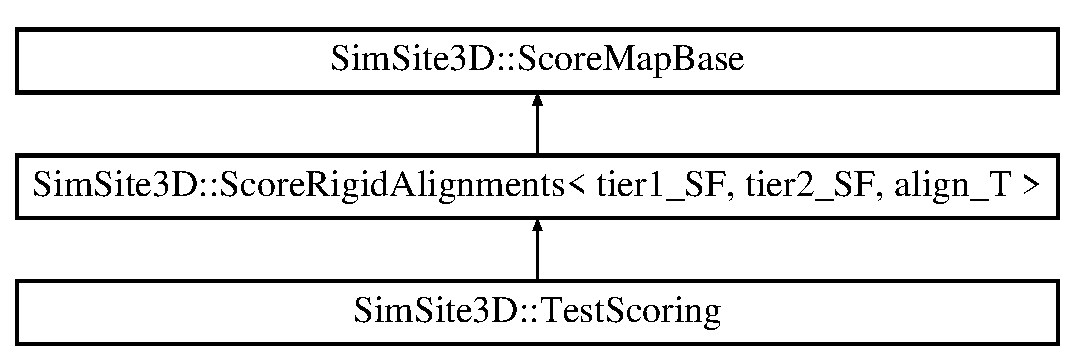
\includegraphics[height=3cm]{classSimSite3D_1_1TestScoring}
\end{center}
\end{figure}
\subsection*{Public Member Functions}
\begin{CompactItemize}
\item 
\bf{Test\-Scoring} (\bf{Model\-Sitemap} $\ast$model\_\-in, const \bf{Search\-Parameters} \&params)
\begin{CompactList}\small\item\em Default constructor for scoring methods of rigidly aligned sitemaps. \item\end{CompactList}\item 
\bf{$\sim$Test\-Scoring} ()\label{classSimSite3D_1_1TestScoring_47bf11af16fb49567855096808ec8a7f}

\begin{CompactList}\small\item\em basic destruction \item\end{CompactList}\end{CompactItemize}
\subsection*{Protected Member Functions}
\begin{CompactItemize}
\item 
my\_\-float\_\-t \bf{score} (const \bf{Dbase\-Sitemap} \&search, rigid\_\-align\_\-vi scores)
\begin{CompactList}\small\item\em Given an alignment of search to the query, score said alignment. \item\end{CompactList}\item 
my\_\-float\_\-t \textbf{correspondences} (my\_\-float\_\-t $\ast$$\ast$query\_\-pts\_\-ptr, my\_\-float\_\-t $\ast$$\ast$db\_\-pts\_\-ptr, size\_\-t $\ast$npts)\label{classSimSite3D_1_1TestScoring_1bce69b267b72ae43cd980caa7fcfd0e}

\end{CompactItemize}
\subsection*{Static Private Attributes}
\begin{CompactItemize}
\item 
static const std::string \bf{\_\-fname} = \char`\"{}Test\-Scoring.C\char`\"{}\label{classSimSite3D_1_1TestScoring_b4ebe268b1b74f5fe669c109de103c8f}

\begin{CompactList}\small\item\em \char`\"{}Weighted\-Sums\-Score.C\char`\"{} \item\end{CompactList}\item 
static const my\_\-float\_\-t \bf{POLAR\_\-SUM\_\-W} = -0.0140894\label{classSimSite3D_1_1TestScoring_d98e1f35e2bdf736d103e6e5b0acb5dd}

\begin{CompactList}\small\item\em -10370 \item\end{CompactList}\item 
static const my\_\-float\_\-t \bf{HPHOBIC\_\-COUNT\_\-W} = 0\label{classSimSite3D_1_1TestScoring_4d97cb87f8816169344f99d6d82f9910}

\begin{CompactList}\small\item\em -4130 \item\end{CompactList}\item 
static const my\_\-float\_\-t \bf{POLAR\_\-MISMATCH\_\-W} = 0\label{classSimSite3D_1_1TestScoring_346e2d0eab2f073e92340f747237e674}

\begin{CompactList}\small\item\em 11428 \item\end{CompactList}\item 
static const my\_\-float\_\-t \bf{UNSAT\_\-POLAR\_\-W} = 0\label{classSimSite3D_1_1TestScoring_668c7fb952beb31eb9c991e0f736570c}

\begin{CompactList}\small\item\em 963 \item\end{CompactList}\item 
static const my\_\-float\_\-t \bf{CONSTANT\_\-TERM} = -0.124725\label{classSimSite3D_1_1TestScoring_1ee5151bf6450adf872d86f51b9f9e72}

\begin{CompactList}\small\item\em -58070 \item\end{CompactList}\item 
static const my\_\-float\_\-t \bf{max\_\-dist} = 1.5\label{classSimSite3D_1_1TestScoring_46212ce7b93b0912702739bfd3efe04f}

\begin{CompactList}\small\item\em 1.5 angstroms \item\end{CompactList}\end{CompactItemize}


\subsection{Detailed Description}
Base class for scoring rigid alignments of dbase sitemaps to a given model. 



\subsection{Constructor \& Destructor Documentation}
\index{SimSite3D::TestScoring@{SimSite3D::Test\-Scoring}!TestScoring@{TestScoring}}
\index{TestScoring@{TestScoring}!SimSite3D::TestScoring@{SimSite3D::Test\-Scoring}}
\subsubsection{\setlength{\rightskip}{0pt plus 5cm}Test\-Scoring::Test\-Scoring (\bf{Model\-Sitemap} $\ast$ {\em model\_\-in}, const \bf{Search\-Parameters} \& {\em params})}\label{classSimSite3D_1_1TestScoring_30cc41f637641ce6dd0c225594e17e15}


Default constructor for scoring methods of rigidly aligned sitemaps. 

\begin{Desc}
\item[Parameters:]
\begin{description}
\item[{\em model\_\-in}]Pointer to the model points (sitemap class) \item[{\em params}]Reference to the search's runtime parameters \end{description}
\end{Desc}


\subsection{Member Function Documentation}
\index{SimSite3D::TestScoring@{SimSite3D::Test\-Scoring}!score@{score}}
\index{score@{score}!SimSite3D::TestScoring@{SimSite3D::Test\-Scoring}}
\subsubsection{\setlength{\rightskip}{0pt plus 5cm}my\_\-float\_\-t Test\-Scoring::score (const \bf{Dbase\-Sitemap} \& {\em search}, rigid\_\-align\_\-vi {\em scores})\hspace{0.3cm}{\tt  [protected]}}\label{classSimSite3D_1_1TestScoring_e0e06721302874c8daff87995f2609b9}


Given an alignment of search to the query, score said alignment. 

\begin{Desc}
\item[Parameters:]
\begin{description}
\item[{\em search}]Pointer to the sitemap aligned to the model sitemap \end{description}
\end{Desc}
\begin{Desc}
\item[Returns:]The score of the alignment \end{Desc}


The documentation for this class was generated from the following files:\begin{CompactItemize}
\item 
TESTSCORING.H\item 
TESTSCORING.C\end{CompactItemize}
